\chapter{Case of Study} \label{expres} 
\section{Experiments}
In this chapter we present the relevant experiments that were done to test the proposed method. Subsequently, it shows the implementation of the method in a adaptive learning environment used as case of study, deployed in different places. A wide explanation of the system interfaces and its functionality is explained also.

In this particular experimental scenario, we propose some guidelines and follows some guidelines from related work like the work of Hervas\cite{bravo2005display}, Chen\cite{Chen2007}, Garcia-Valdez\cite{mariotesis}, and they are briefly explained next.
\begin{itemize}	

\item • Hypothesis: before running the experiment we must form an hypothesis. It is important to be concise and restrictive about this hypothesis, and design an experiment that tests the hypothesis. For example, an hypothesis can be that adaptive environment A adapts and presents better learning objects to the user and the user likes and learn more than the environment B. In that case,the experiment should test the acceptance and assimilation of the environment including content, ease of use etc.

\item • Controlling variables: when comparing a few learning environments on a certain hypothesis, it is important that all variables that are not tested will
stay fixed. For example, suppose that we wish to compare the acceptance and assimilation of the environment A and environment B, that both use
different technologies. 

\item • Generalization power: when drawing conclusions from experiments, we may desire that our conclusions generalize beyond the immediate context of the experiments. When choosing an environment for a real application, we may want our conclusions to hold on the deployed system. Generally speaking, the more diverse the data used, the more it can generalize the results.
\end{itemize}

The next sections show a comprehensive description of the experimental setup for experiments, as well as results obtained in the experiments. Each method was tested
using different topics and context. This chapter ends with the description of the functionality of the prototype used to validate the method utilized in the experiments.

\section{Adaptive Learning Environment topic 1}
In earlier implementations of the adaptive environment several experiments were done to test the behavior and the performance. For the experiment the proposed hypothesis is The acceptance and accuracy of the content showed in the adaptive learning environment. The first experiment presents and adaptive learning environment used to teach the topic "El himno nacional Mexicano". llevado a cabo en las instalaciones del instituto tecnologico de tijuana. 
\subsection{Devices}
Los dispositivos usados en este experimento se describen a continuacion. Se necesito de un servidor para manejar las peticiones, almacenar los objetos de aprendizaje, generar la secuencia de aprendizaje y mantener el servicio web activo. En este caso el servidor era una computadora Gateway fx6850 el cual cuenta con 12gb de ram y procesador intel i7 de segunda generacion. se utilizaron 3 monitores de diferentes resoluciones el primero de 1440x900 pixeles, el segundo de 1600x900 y el tercero de 1980x1080 pixeles. Lo que genero un problema a la hora de desplegar imagenes o videos pero se tomaron medidas para adaptar el contenido a diferentes resoluciones. Una tablet nexus7 con la cual el usuario podia controlar la navegacion entre actividades y contestar algunos cuestionarios. y audifonos para el sonido.

\begin{figure}[ht!]  
\centering  
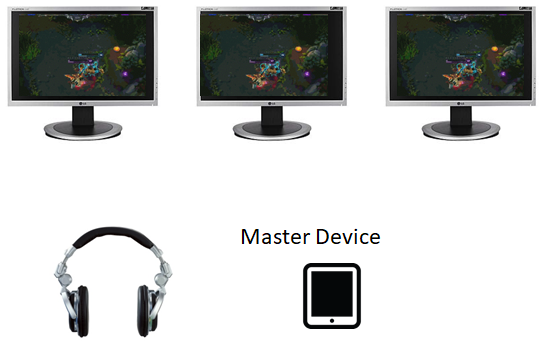
\includegraphics[scale=1]{ambiente2}
\quad  
\caption{Configuration of the first adaptive environment}  
\label{ambiente2}  
\end{figure}
  

\subsection{Topic/Content}
Seleccionamos el tema de el himno nacional mexicano por la razon de que nos parecio un tema de interez general y por lo tanto digerible para diferentes edades y personas.
se comenzo con una breve historia del himno nacional involucrando a sus autores tanto de musica como de letra y una breve sinopsis de cada uno de ellos en la figura \ref{Nuno2} podemos observar una imagen con los 2 personajes pero se muestran 2 imagenes de cada una de los autores, dependiendo del usuario se muestra una u otra imagen.
\begin{figure}[ht!]  
\centering  
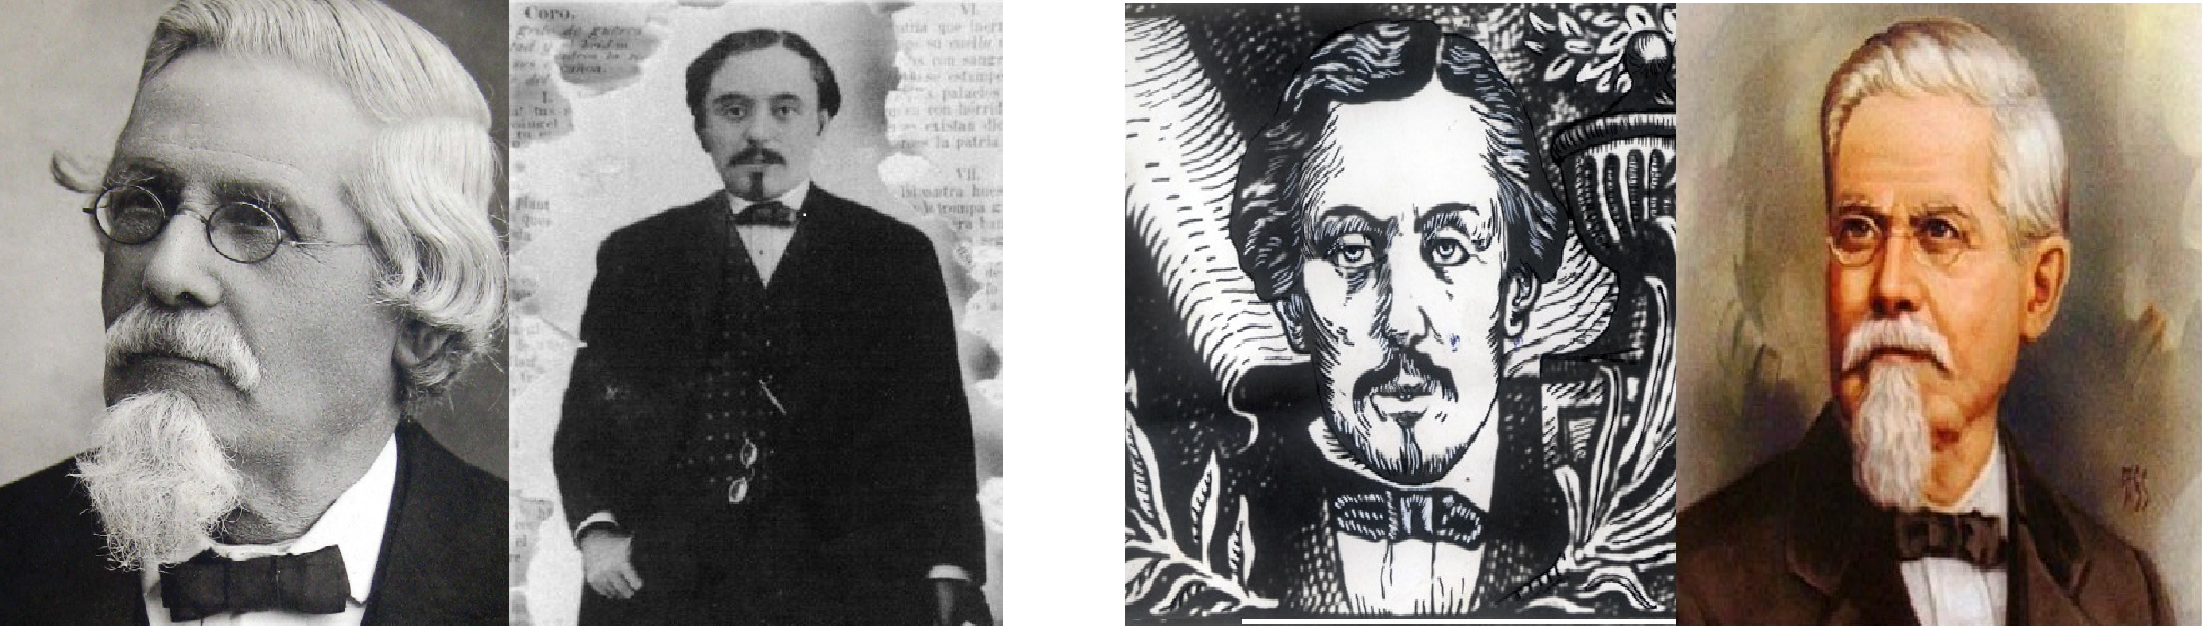
\includegraphics[scale=.25]{Jaime_Nuno2}
\quad  
\caption{2 learning objects.}  
\label{Nuno2}  
\end{figure}

Como lo mencionamos se manejan 3 tipos de usuarios tomando como referencia su edad. basado en el rando de edad un sistema difuso elige que contenido mostrar al usuario. en la imagen anterior \ref{Nuno2} se muestran las imagenes de los autores del himno nacional pero para el tipo de usuario 2 y 3. dependiendo del tipo de usuario cada una de las actividades puede cambiar y hacerce un poco mas digerible, por ejemplo para el usuario 3 que se supone un usuario mas metodico y que tiene en su mayoria tiene mejor aceptacion de informacion compleja se le muestra mas texto, graficas y tablas que quiza son mas dificiles de entender para los usuarios 1 y quiza al usuario 2. entonces es la misma actividad de aprendizaje pero con pequeños cambios con respecto a los diferentes usuarios. 

\subsection{Users}
Los usuarios para este experimento fue una muestra de compañeros de laboratorio, maestros, amigos e hijos de compañeros un grupo de usuarios 10 de diferentes perfiles (tabla 1) con el prototipo del ambiente para ver la impresión que tuvieron realizar una actividad de aprendizaje y obtener retroalimentación de ellos. Este ambiente está planeado para usarse en aéreas grandes pero en este caso se uso un espacio pequeño para la prueba. Para este caso solo se tomaron la edad y el nivel académico el cual va desde 1 hasta 21 donde 1 es primer año de primaria y 21 tiene grado de doctor como lo podemos observar en la tabla \ref{tab:users1}.

\begin{table}
\centering
\small
\captionsetup{font=footnotesize}
\caption{List of users participating in the experiment.}
\label{tab:users1} 

\small
\begin{tabular}{p{3cm} p{3cm} p{3cm} }
\hline{\smallskip}
User & Age	& Academic level\\
\noalign{\smallskip}\hline\noalign{\smallskip}
\small{	1	}& \small{	6	}& \small{	1	}\\
\small{	2	}& \small{	48	}& \small{	19	}\\
\small{	3	}& \small{	23	}& \small{	17	}\\
\small{	4	}& \small{	23	}& \small{	18	}\\
\small{	5	}& \small{	23	}& \small{	18	}\\
\small{	6	}& \small{	24	}& \small{	17	}\\
\small{	7	}& \small{	31	}& \small{	19	}\\
\small{	8	}& \small{	35	}& \small{	20	}\\
\small{	9	}& \small{	45	}& \small{	21	}\\
\small{	10	}& \small{	29	}& \small{	19	}\\
\hline

\end{tabular}
\end{table}

\subsection{Survey}

Cuando los usuarios terminaron de utilizar el ambiente se les realizo una pequeña encuesta, esta encuesta consistía en 5 preguntas sobre su experiencia al utilizar el ambiente preguntas como si se le dificulto utilizarlo o si fue de su agrado los recursos mostrados, con el objetivo de obtener retroalimentación de los usuarios para hacer futuras mejoras y modificaciones que se muestra en la tabla \ref{users2}.
\begin{table}
\small
\centering
\captionsetup{font=footnotesize}
\caption{List of users participating in the experiment.}
\label{tab:users2} 

\small
\begin{tabular}{p{12cm} p{4cm} }
\hline\noalign{\smallskip} 
Question & Answers \\
\noalign{\smallskip}\hline\noalign{\smallskip}\hline
\small{1.From 1-10 how easy it was use the environment? } & \small{1-10[  ]} \\ \hline  
\small{2.From 1-10, how was your satisfaction about the information displayed in the environment? } & \small{1-10[  ]} \\ \hline
\small{3.Did you like the idea of using various visual elements?  } & \small{1. Yes 2.No} \\ \hline 
\small{4.Was necessary technical assistance to use the environment?   } & \small{1. Yes 2.No} \\ \hline   
\small{5.Would you recommend the use of this environment to others?  } & \small{1. Yes 2.No} \\ \hline 
\hline
\noalign{\smallskip}\hline
\end{tabular}
\end{table}

\section{Adaptive Learning Environment topic 2}
For this part of the study users immersed in an exhibitor that gave them visual and aural information as shown in Figure \ref{fig:environment} on a topic selected based on various criteria, such as the location of the study on this occasion was a interactive museum and the festival of children’s day approaching we try to use a simple theme and it will bring awareness so we decided to use the theme of water where information was displayed as the uses of the same, its cycle, forms of energy that could generate, health, and the importance of it for the planet. Each of users are generating an account on the system to register their activity, after that we were made a brief explanation of how it worked the exhibitor others based on observation no longer required this explanation. The user took a tablet that was the how the user interacted with the exhibitor, with which had control of the flow of information, as the information was a sequence at the end of the last activity was a questionnaire on the information received besides a survey.

\begin{figure}[htbp]
\centering
\subfigure[User interacting with the environment.]{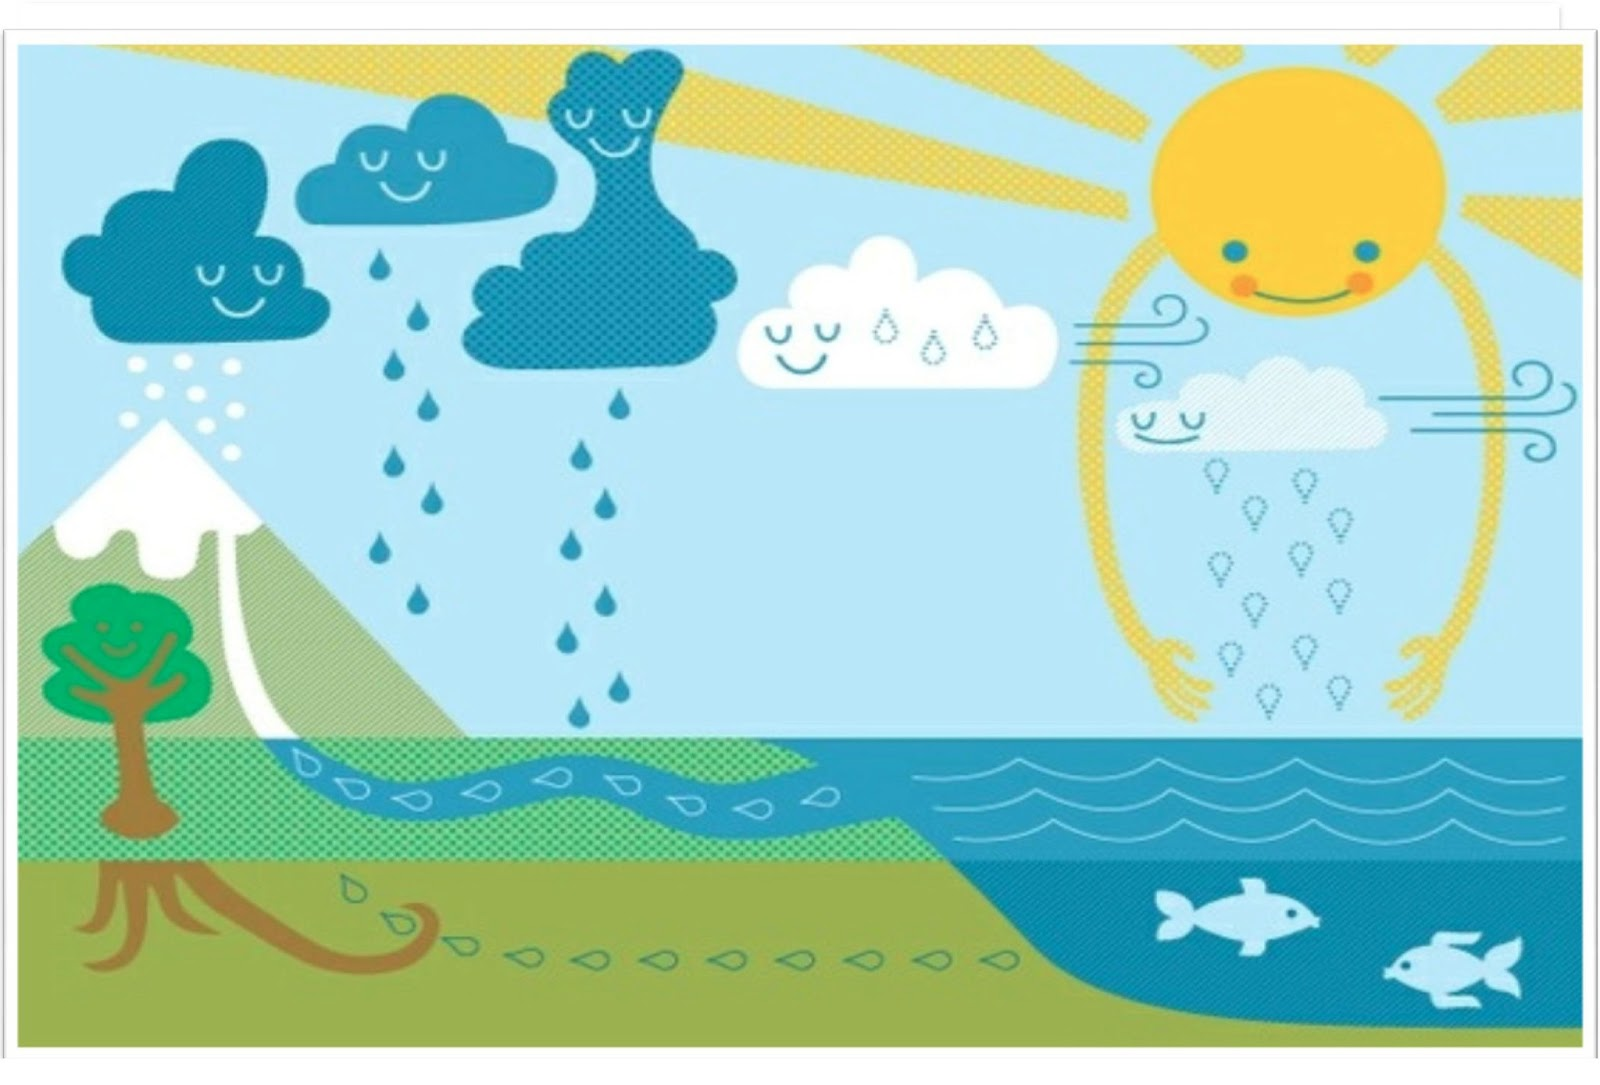
\includegraphics[width=40mm]{agua}}\hspace{10mm}
\subfigure[Front view of the equipt.]{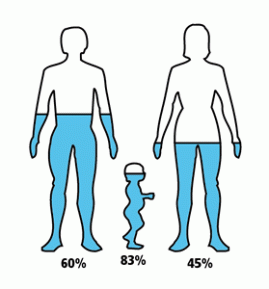
\includegraphics[width=40mm]{agua3}}{10mm}
\caption{The environment.} \label{fig:environment}
\end{figure}

\subsection{Devices}
Los dispositivos usados en este experimento se describen a continuacion. Se necesito de un servidor para manejar las peticiones, almacenar los objetos de aprendizaje, generar la secuencia de aprendizaje y mantener el servicio web activo. En este caso el servidor era una computadora Mac Pro 2014 la cual cuenta con 12gb de ram y procesador intel xeon. se utilizaron 3 proyectores de las mismas resoluciones a diferentes tamaños organizados como se puede observar en la figura \ref{trompo1}. una computadora adicional que realizo diversas tareas como mostrar el contenido de 2 proyectores y reproducir el audio,  una laptop para mostrar contenido en el tercer proyector y una laptop mas donde para obtener los datos del sensor kinect. 

\begin{figure}[ht!]  
\centering  
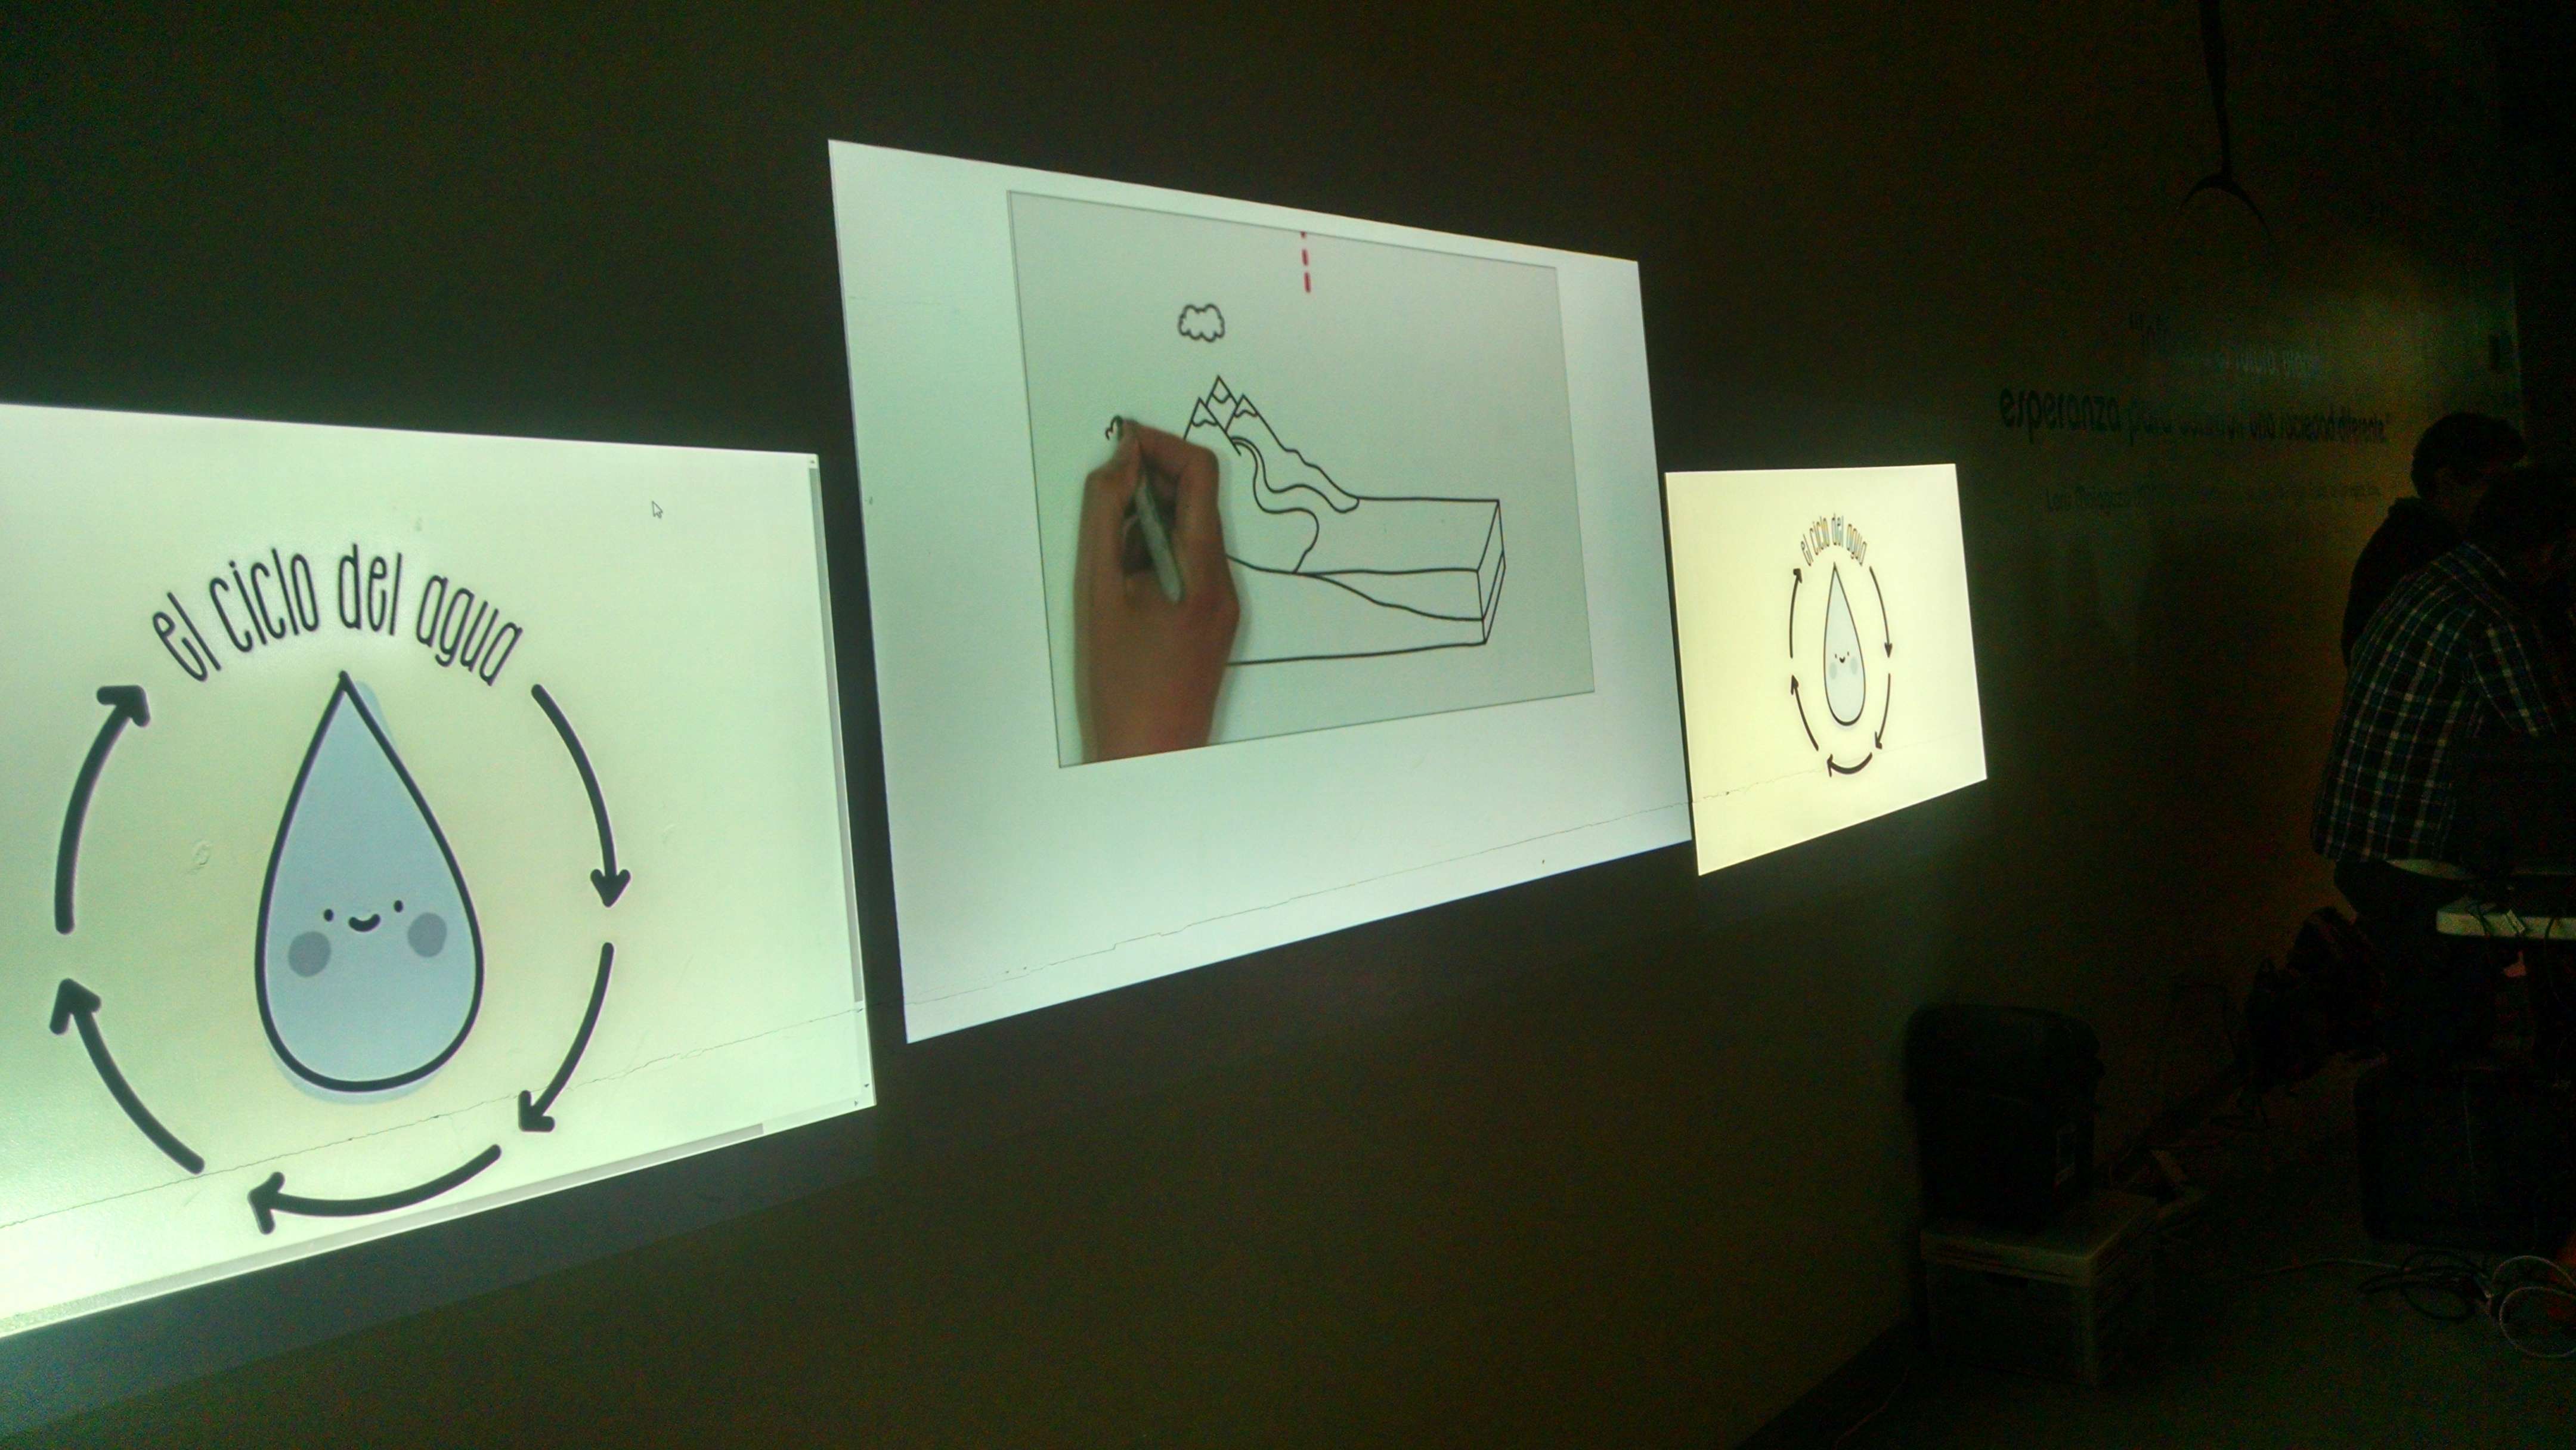
\includegraphics[scale=.08]{trompo1}
\caption{Front view of the environment.}  
\label{trompo1}  
\end{figure}
Una tablet nexus7 con la cual el usuario podia controlar la navegacion entre actividades y contestar algunos cuestionarios. y audifonos para el sonido. ademas del sensor kinekt 2 para sensar al usuario.


\subsection{Topic/Content}
Para este experimento la eleccion del tema fue influenciada por el lugar y la fecha donde se llevaria a cabo el lugar fue el museo interactivo el trompo de tijuana a pocos dias del el dia festivo "El dia del Niño" por lo que optamos por elegir un tema digerible y que haga conciencia en los usuarios. El tema elegido fue "el Cuidado del agua" donde se recabaron al rededor de 23 diferentes imagenes, 8 audios, 1 video en la figura \ref{fig:agua}. 
\begin{figure}[htbp]
\centering
\subfigure[water percent of the body]{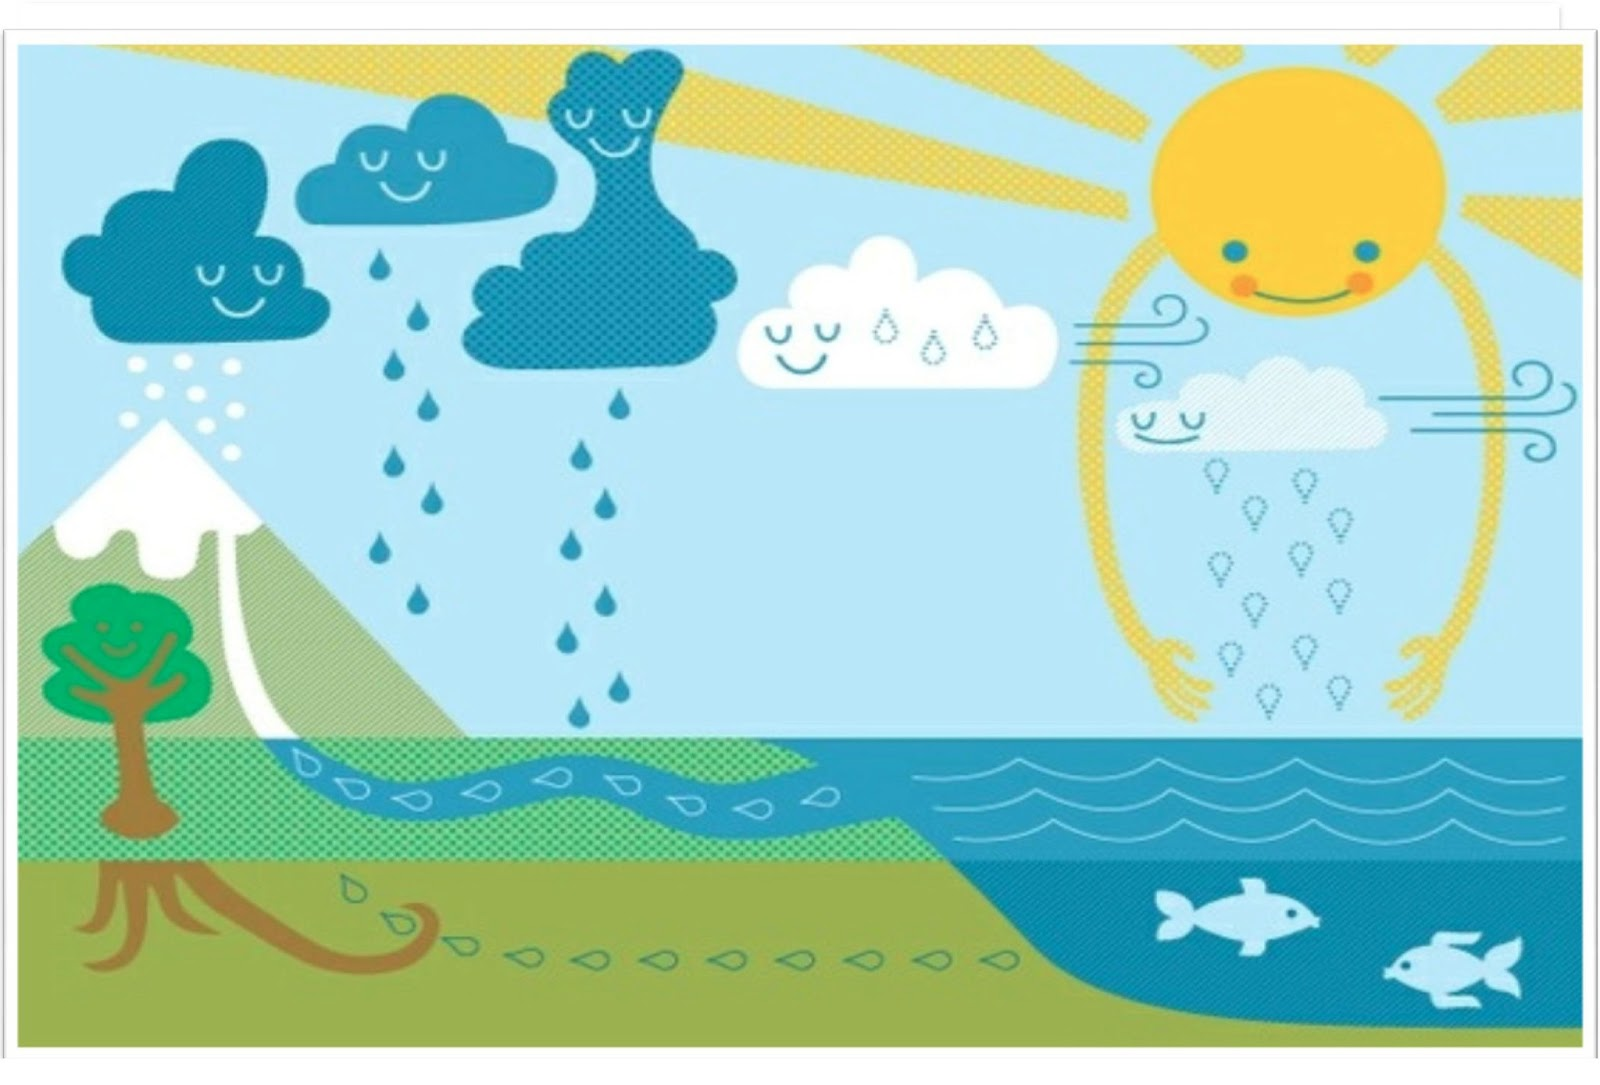
\includegraphics[width=40mm]{agua}}\hspace{10mm}
\subfigure[ciclio del agua]{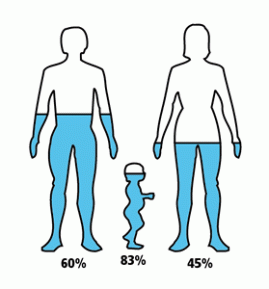
\includegraphics[width=40mm]{agua3}}\vspace{10mm}
\subfigure[total de agua en el planeta]{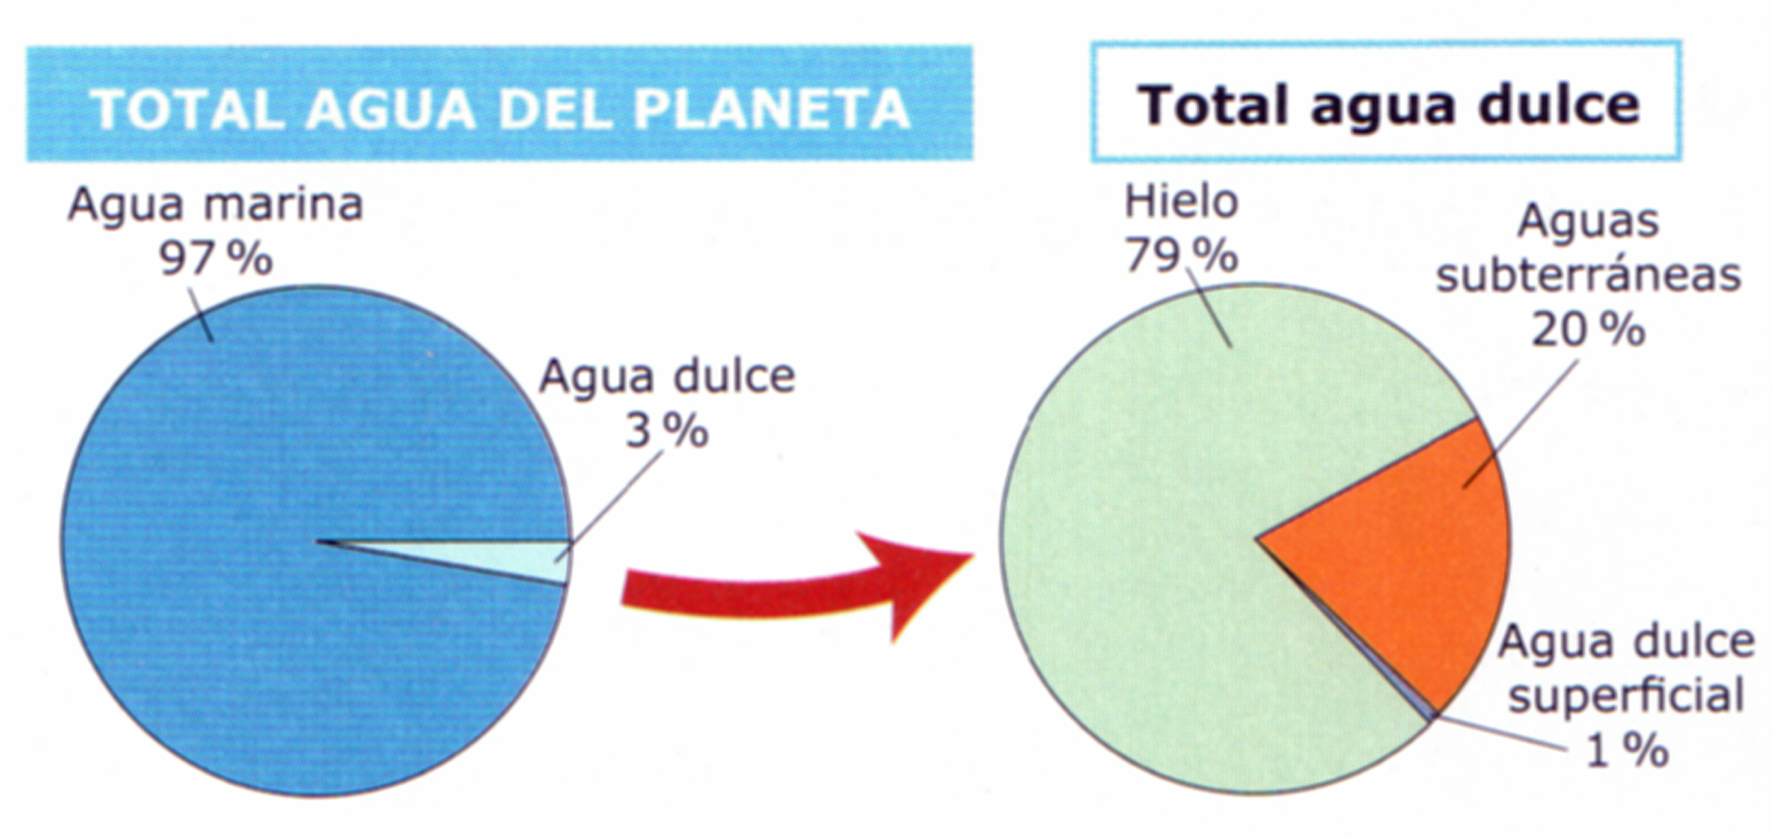
\includegraphics[width=80mm]{agua2}}
\caption{imagenes usadas en la secuencia de aprendizaje.} \label{fig:agua}
\end{figure}

La informacion mostrada por la actividad fue desde el ciclo del agua, su importacia para nuestra salud, la energia producida por la misma, ademas de el cuidado que hay que tener con ella y como evitar la contaminacion. La actividad se podia completar entre 8 y 10 minutos dependiendo de los recursos mostrados a los diferentes usuarios como lo podemos ver en la figura \ref{exp2}.

\begin{figure}[ht!]  
\centering  
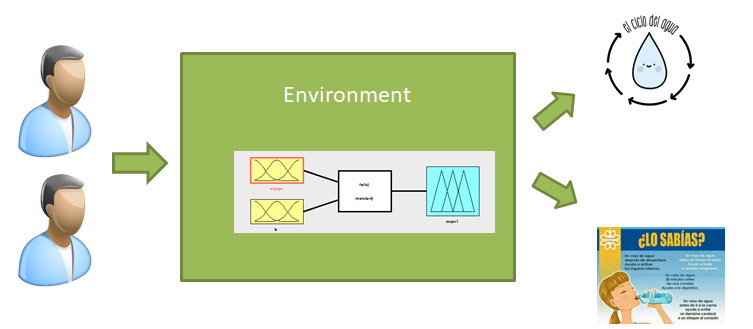
\includegraphics[scale=.5]{exp2}
\caption{How to choose content to show.}  
\label{exp2}  
\end{figure}

\subsection{Users}
This experiment was conducted with visitors of the museum’s "El trompo" where 21 users divided into 2 groups participated, the first has 10 users between 6 and 11 years 50\% men and 50\% women and the second group consisted of 11 users over 11 years old  66\% men 44\% women en la tabla \ref{tab:users21} y en la tabla \ref{tab:users22} se pueden observar algunos datos adicionales de los 2 grupos de usuarios, nota adicional algunos usuarios no quisieron revelar su edad o nombre por lo que se les respeto su desicion y se les dejo con el signo de ? y la minoria hablaba otro idioma lo que puso a prueba el contenido ya que este estaba totalmente en español aunque los usuarios aun asi participaron.
\begin{table}
\small
\centering
\captionsetup{font=footnotesize}
\caption{List of users participating in the experiment group 1.}
\label{tab:users21} 
\small
\begin{tabular}{p{3cm} p{3cm} p{3cm} }
\hline{\smallskip}
User & Name	& Age\\
\noalign{\smallskip}\hline\noalign{\smallskip}
\small{	1	}& \small{	Jose 	}& \small{	?	}\\
\small{	2	}& \small{	Mariof	}& \small{	?	}\\
\small{	3	}& \small{	Jaqueline	}& \small{	?	}\\
\small{	4	}& \small{	? 	}& \small{	10	}\\
\small{	5	}& \small{	Alondra	}& \small{	38	}\\
\small{	6	}& \small{	Josue 	}& \small{	10	}\\
\small{	7	}& \small{	Mario	}& \small{	14	}\\
\small{	8	}& \small{	Cinthya	}& \small{	30	}\\
\small{	9	}& \small{	Brisa	}& \small{	11	}\\
\small{	10	}& \small{	Hector 	}& \small{	37	}\\
\small{	11	}& \small{	Enrique	}& \small{	12	}\\
\hline
\end{tabular}
\end{table}
 
\begin{table}
\small
\centering
\captionsetup{font=footnotesize}
\caption{List of users participating in the experiment group 2.}
\label{tab:users22} 
\small
\begin{tabular}{p{3cm} p{3cm} p{3cm} }
\hline{\smallskip}
User & Name	& Age\\
\noalign{\smallskip}\hline\noalign{\smallskip}
\small{	1	}& \small{	Josue	}& \small{	8	}\\
\small{	2	}& \small{	Kevin	}& \small{	9	}\\
\small{	3	}& \small{	Monserrat	}& \small{	7	}\\
\small{	4	}& \small{	Evelin	}& \small{	9	}\\
\small{	5	}& \small{	Armando	}& \small{	8	}\\
\small{	6	}& \small{	Jorge	}& \small{	7	}\\
\small{	7	}& \small{	Gemma	}& \small{	8	}\\
\small{	8	}& \small{	Perla	}& \small{	8	}\\
\small{	9	}& \small{	Quetzal	}& \small{	7	}\\
\small{	10	}& \small{	?	}& \small{	6	}\\
\hline

\end{tabular}
\end{table}
\subsection{Survey}
Cuando los usuarios terminaron de utilizar el ambiente se les realizo una pequeña encuesta, dependiendo del usuario se le aplico una u otra encuesta que podemos observar en la tabla \ref{tab:users1} y la tabla \ref{tab:users2} respectivamente.
\begin{table}
\small
\centering
\captionsetup{font=footnotesize}
\caption{Survey to the user group 1.}
\label{tab:users2} 

\small
\begin{tabular}{p{12cm}}
\hline\noalign{\smallskip} 
Question \\
\noalign{\smallskip}\hline\noalign{\smallskip}\hline
\small{1.Did you like what you saw in the activity you just did? } \\ 
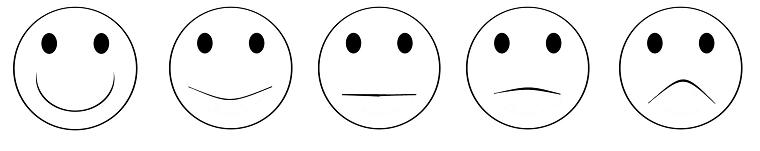
\includegraphics[width=5cm]{likert}\\ \hline  
\small{2.Did you like watching different pictures and videos? }  \\ 
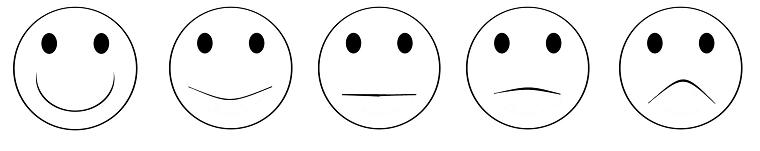
\includegraphics[width=5cm]{likert}\\ \hline 
\small{3.Was it easy to use the station?  } \\ 
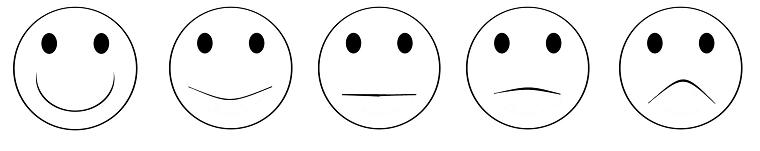
\includegraphics[width=5cm]{likert}\\ \hline  
\small{4.Did you have fun using the station?   } \\ 
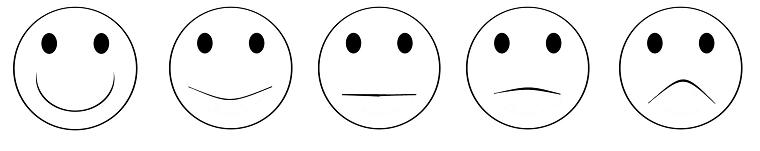
\includegraphics[width=5cm]{likert}\\    

\hline
\noalign{\smallskip}\hline
\end{tabular}
\end{table}

\begin{table}
\small
\centering
\captionsetup{font=footnotesize}
\caption{Survey to the user group 2.}
\label{tab:users2} 

\small
\begin{tabular}{p{12cm}}
\hline\noalign{\smallskip} 
Question \\
\noalign{\smallskip}\hline\noalign{\smallskip}\hline
\small{1.I found useful for my learning this station? } \\ 
\small{	1			2			3			4			5	}\\\hline
\small{2.Using this station allowed me to learn more things faster? }  \\ 
\small{	1			2			3			4			5	}\\\hline
\small{3.The use of several images increased my understanding of the subject?  } \\ 
\small{	1			2			3			4			5	}\\\hline
\small{4.It was easy for me to use the station?   } \\ 
\small{	1			2			3			4			5	}\\\hline
\small{5.I can explain to someone how to use the station? } \\ 
\small{	1			2			3			4			5	}\\\hline
\small{6.Using this station allowed me to learn more things faster? }  \\ 
\small{	1			2			3			4			5	}\\\hline
\small{7.I think that including this station in the museum was a good idea  } \\ 
\small{	1			2			3			4			5	}\\\hline
\small{8.I liked to use the station   } \\   
\small{	1			2			3			4			5	}\\\hline
\noalign{\smallskip}\hline
\end{tabular}
\end{table}

\section{Adaptive Learning Environment topic 3}
Este experimento se llevo acabo en las instalaciones del tecnologico de tijuana ajustando nuestro prototipo con la retroalimentacion del segundo experimento. Para poder atender mas usuarios en esta ocacion las actividades fueron las mismas para todos esto permitio una mejor lectura de datos a los usuarios y minimizo el tiempo de uso de cada usuario en la actividad.This study was very similar to the last one that had some small modifications and additions, now the user no longer had control flow only observe and also to observe the user now will take video and sensor, the theme of the exhibition were video games and film as the age of the users would go for almost 17 years and older could be topics of their interest. In the same way as in the first part each user had an account to record the activity only this occasion the data produced by the sensor and videos captured by the camera would be recorded, and in the same way as in the first part at the end we surveyed the users.
For the first part of the study we get data from the survey conducted at the end, in the second they are collected and used data from sensors, this data were a bit more complex, first we need an observer to evaluate the user manually, where the observer determined whether the user was putting attention to what he saw or distracted and based on that assigned a level of attention on a scale of 1 to 3 where 1 is little attention 2 average attention and 3 very attentive. 
\subsection{Devices}
Los dispositivos usados en este experimento se describen a continuacion. Se necesito de un servidor para manejar las peticiones, almacenar los objetos de aprendizaje, generar la secuencia de aprendizaje y mantener el servicio web activo. En este caso el servidor era una computadora Mac Pro 2014 la cual cuenta con 12gb de ram y procesador intel xeon. se utilizaron 3 proyectores de las mismas resoluciones a diferentes tamaños organizados como se puede observar en la figura \ref{ambiente4}. una computadora adicional que realizo diversas tareas como mostrar el contenido de 2 proyectores y reproducir el audio,  una laptop para mostrar contenido en el tercer proyector y una laptop mas donde para obtener los datos del sensor kinect.
\begin{figure}[ht!]  
\centering  
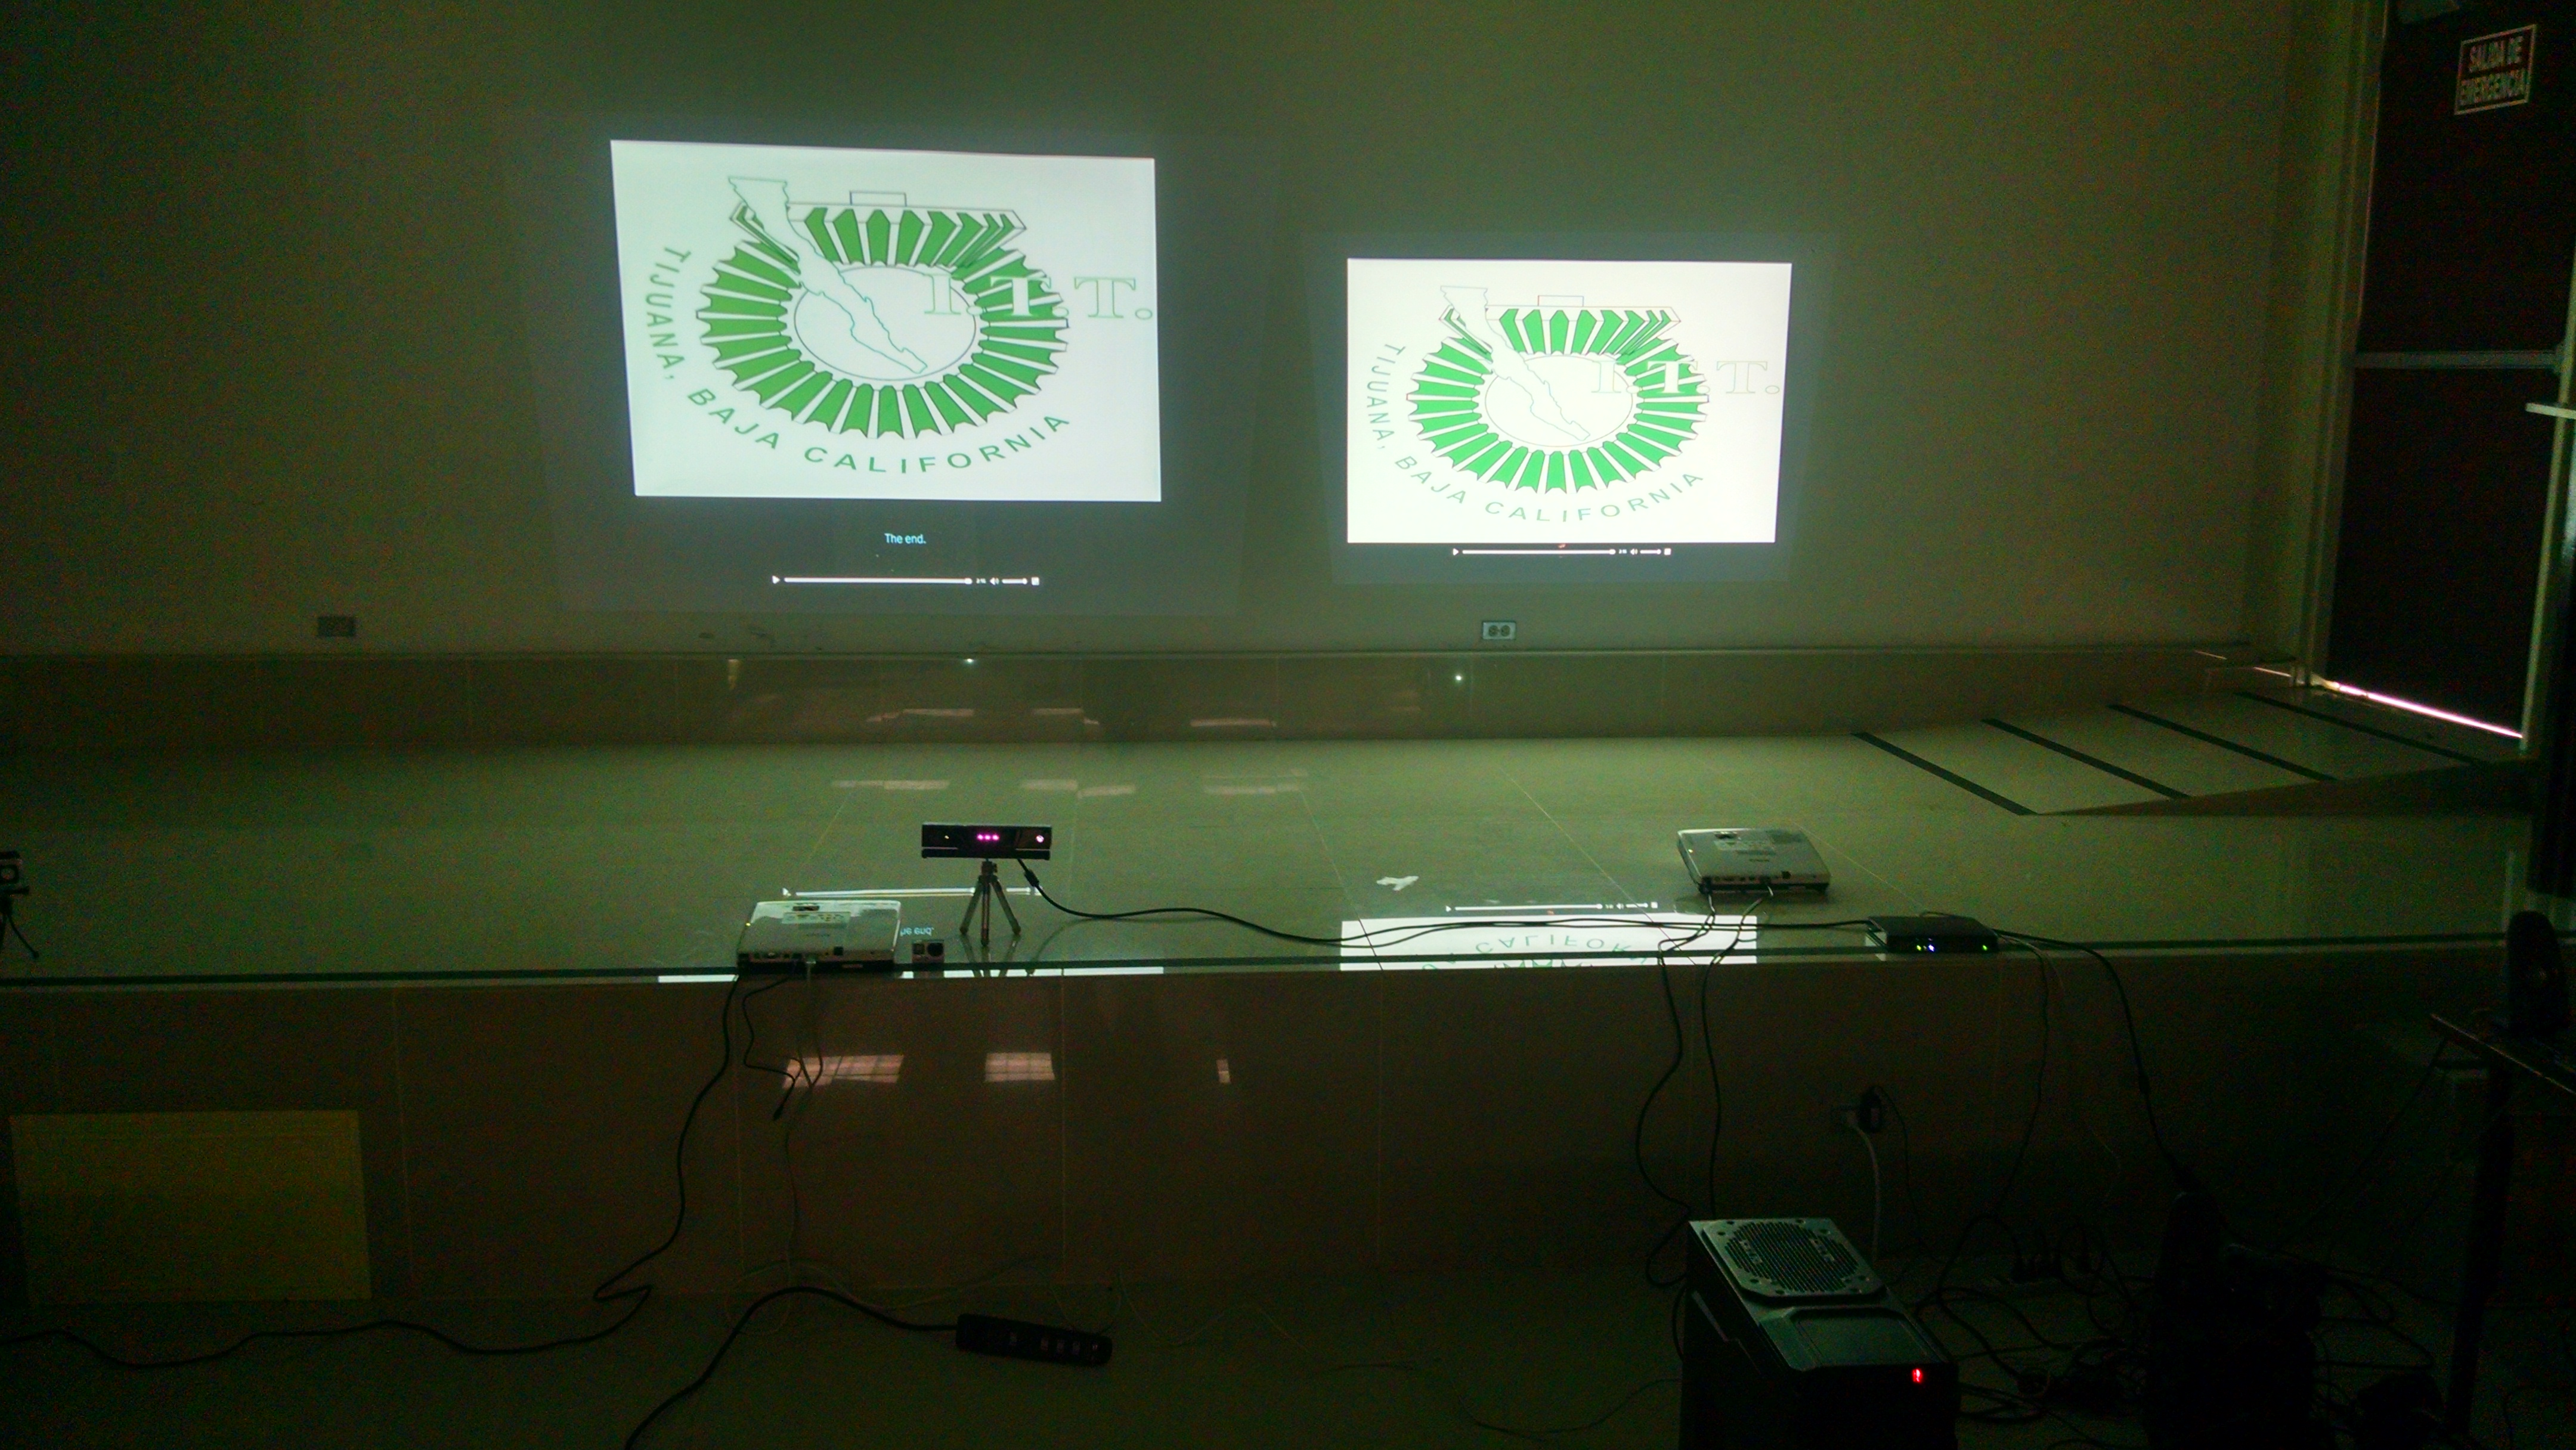
\includegraphics[scale=0.08]{tec1}
\quad  
\caption{Configuration of the last adaptive environment}  
\label{ambiente4}  
\end{figure}

\subsection{Topic/Content}
PAra elegir el tema a mostrar en el ambiente decidimos optar por temas de interez para poblacion de usuarios que fueron video juegos y el cine. el video sobre los video juegos fue sobre el video juego league of legends y el video de cine fue una explicacion de la trilogia de starwars en 2 minutos con legos.
\subsection{Users}
Participaron un total de 41 users of the Technological Institute of Tijuana were used aged between 18 and 50 years 66 \% men 34 \% women. 
\subsection{Survey}

 Cuando los usuarios terminaron de utilizar el ambiente se les realizo una pequeña encuesta que se muestra a continuacion.

\begin{table}
\small
\centering
\captionsetup{font=footnotesize}
\caption{Survey to the user group.}
\label{tab:users2} 

\small
\begin{tabular}{p{12cm}}
\hline\noalign{\smallskip} 
Age:\_\_\_\_\_\_\_\_\_\_\_\_ \\
Video 1 \\
\noalign{\smallskip}\hline\noalign{\smallskip}\hline
\small{1.How much did you like the video 1? } \\ 
\small{	1			2			3			4			5	}\\\hline
\small{2.How much did you like the main video? }  \\ 
\small{	1			2			3			4			5	}\\\hline
\small{3.How much did you like the complementary video?  } \\ 
\small{	1			2			3			4			5	}\\\hline
\hline\noalign{\smallskip} 
Video 2 \\
\noalign{\smallskip}\hline\noalign{\smallskip}\hline
\small{1.How much did you like the video 1? } \\ 
\small{	1			2			3			4			5	}\\\hline
\small{2.How much did you like the main video? }  \\ 
\small{	1			2			3			4			5	}\\\hline
\small{3.How much did you like the complementary video?  } \\
\small{	1			2			3			4			5	}\\\hline 
\hline\noalign{\smallskip} 

\small{How often do you use video games?   } \\ 
\small{	1			2			3			4			5	}\\\hline
\small{How often do you go to the cinema? } \\ 
\small{	1			2			3			4			5	}\\\hline
\hline\noalign{\smallskip} 
To play you like \\
\noalign{\smallskip}\hline\noalign{\smallskip}\hline
\small{6.Using this station allowed me to learn more things faster? }  \\ 
\small{	Phone 	1			2			3			4			5	}\\\hline
\small{	Tablet 	1			2			3			4			5	}\\\hline
\small{	PC	 	1			2			3			4			5	}\\\hline
\small{	Console		1			2			3			4			5	}\\\hline

\small{Mention 2 of your favorite video games.   } \\   
\small{		}\\\hline
\small{		}\\\hline
\small{1.How much did you like Star Wars? } \\ 
\small{	1			2			3			4			5	}\\\hline
\small{2.How much did you like Legos? }  \\ 
\small{	1			2			3			4			5	}\\\hline
\small{3.Did you like the way the information was presented?  } \\
\small{	1			2			3			4			5	}\\\hline 
\noalign{\smallskip}\hline
\end{tabular}
\end{table}



